\documentclass[a4paper,12pt, openany]{book}
\usepackage[utf8]{inputenc}
\usepackage[margin=1in]{geometry}
\usepackage[toc]{appendix}
\usepackage{graphicx}
\usepackage{hyperref}
\usepackage{float}
\usepackage{setspace}
\usepackage{mathptmx}
\usepackage{tkz-berge}
\usepackage{csquotes}
\usepackage{array}
\usepackage{caption} 
\usepackage[htt]{hyphenat}
\usepackage{amsmath,amssymb}
\usepackage{subcaption}
\usepackage[export]{adjustbox}
\usepackage{pdfpages}
\usepackage{filecontents}

\usepackage{fancyhdr} 

\usepackage[style=ieee]{biblatex}
\addbibresource{references.bib}


\usepackage{sectsty}
%\chapternumberfont{\normalsize} 
\chaptertitlefont{\LARGE}


\title{Project Report}
\author{Loïc Fonkam}
\date{this month, 2019}

\makeatletter
\renewcommand*{\ext@figure}{lot}
\let\c@figure\c@table
\let\ftype@figure\ftype@table
\let\listoftableandfigures\listoftables
\renewcommand*\listtablename{List of Tables and figures}
\makeatother

\begin{document}
\thispagestyle{empty}
\linespread{1.25}      % 1.5 line spacing
\begin{center}
	\begin{LARGE}
		 UNIVERSITY OF BUEA
	\end{LARGE}
	\bigbreak
	\vspace*{0.5in}
	Faculty of Science \\[.5cm]
	
	Department of Computer Science
	
	
	
	\begin{center}
		
		
		\vspace*{0.8in} 
		\begin{LARGE}
			\begin{doublespace}
					 BACHELOR OF SCIENCE IN COMPUTER SCIENCE
			\end{doublespace}

		\end{LARGE}  
	\bigbreak
		Project Report\\[.2cm]
		\begin{Large}
			Dynamic Hash Tables: A Simple Comparison of the Dictionary and Logarithmic Methods.
		\end{Large}\bigbreak
		
		
		
	\end{center}
	
	
	
	
	\begin{center}
		
		
		\vspace*{1in}
		
		\textsc{ AWA FONKAM BRANDON LOIC } \\
		\textsc{SC16A648}
		
		
		
		
		
		
		\vspace*{0.7in}  \textbf{Supervisor} \\
		\vspace{0.1in}  William S. Shu, PhD.
	
		\vspace*{1.3in}
		{\large September 2019}
	\end{center}
\end{center}

\pagenumbering{roman}
\newpage
\vspace*{1in}
\setcounter{page}{1}
\vspace*{0.1\textheight}
\begin{center}
	\section*{DECLARATION}
	\vspace*{.2in}
\end{center}
I hereby declare on my honour that this project report has been written by me, that to the best of my knowledge all borrowed ideas and materials have been duly acknowledged, and that it has not received any previous academic credit at this or any other institution.\\[1cm]

\begin{tabular}{l}
	\makebox[2.8in]{\hrulefill}\\
	
	\hspace*{0mm}\textsc{AWA FONKAM BRANDON LOIC}\\
	\hspace*{0mm}\textsc{SC16A648}\vspace{.5in}\\
	
	\hspace*{0mm}{Department of Computer Science}\\
	\hspace*{0mm}{Faculty of Science}
	
	
\end{tabular}
\addcontentsline{toc}{section}{Declaration}

\newpage
\vspace*{0.25\textheight}
\addcontentsline{toc}{section}{Certification}
\begin{center}
	\section*{CERTIFICATION}
	\vspace*{.2in}
\end{center}
\thispagestyle{empty}

This is to certify that this report entitled “DYNAMIC HASH TABLES: A SIMPLE COMPARISON OF THE DICTIONARY AND LOGARITHMIC METHODS” is the original work of AWA FONKAM BRANDON LOIC with Registration Number SC16A648, student of the Department of
Computer Science at the University of Buea. All borrowed ideas and materials have been duly
acknowledged by means of references and citations. The report was supervised in accordance with the
procedures laid down by the University of Buea. It has been read and approved by:
\\[1.0cm]

\begin{tabular}{lcc}
	\makebox[2.4in]{\hrulefill} & \hspace*{.5in}& \makebox[2in]{\hrulefill}\\
	
	\hspace*{0mm}William S. Shu, PhD CEng CITP MBCS
	&\hspace*{1in}& Date\\[2cm]
	
	\makebox[2.4in]{\hrulefill} & \hspace*{1in} & \makebox[2in]{\hrulefill}\\
	Dr Denis L. Nkweteyim\\
	Head of Department of Computer Science &\hspace*{.5in}
	&
	Date\\
	
\end{tabular}

\newpage
\vspace*{0.25\textheight}
\addcontentsline{toc}{section}{Dedications}
\begin{center}
	\section*{Dedications}
		\vspace*{.2in}
\end{center}

I would like to dedicate this study to my beloved parents, who have been my source of inspiration and gave me strength when I thought of giving up in a period of ill health, who continually provide their moral, spiritual, emotional, and financial support.\bigbreak
To my loving brothers, sisters, relatives, mentor, friends, and classmates who shared their words of advice and encouragement to finish this study.\bigbreak
And lastly, I dedicated this study to the Almighty God. Thank you for the guidance, strength, power of the mind, protection and skills, and for giving me a healthy life. All of these, I offer to you. 



\newpage
\vspace*{0.25\textheight}
\begin{center}
	\section*{Acknowledgement}     
	\vspace*{.3in}
                      \end{center}

I would like to express some special thanks first of all to the LORD ALMIGHTY GOD for the guidance, grace and strength he has always provided me.

Then, I would like to express special gratitude to my lecturer and supervisor Dr William S. Shu, whose valuable guidance has helped me patch this project and make it a proof of success. His suggestion and instructions have served as the major contributor towards the completion for the project. 

I would also like to thank dearly all my lecturers who taught and transferred to me all necessary tool-set of skills. Special thanks to my HOD Dr Denis Lemongew Nkweteyim, Dr Joan Beri Ali Wacka for her tough guidance and Dr Nyamsi Madeleine for being such a great lecturer.

Finally, I would like to thank my loving family and friends, most especially my friends Bomen Tchouagueng and Massina Eloundo whose encouragements and assistance during times of ill health cannot go unforgotten.  

\addcontentsline{toc}{section}{Acknowledgement}

\newpage
\vspace*{0.25\textheight}
\begin{center}
	\section*{Abstract}
	\vspace{.2in}
\end{center}
	Dynamic hash tables provide fast storage and retrieval of data in memory. This fast storage is very important in the development of efficient programs. But, there is a limitation(amount of available RAM) on how much data can be stored in memory. This limitation available in dictionary hash tables was solved by introducing logarithmic hash tables which could index data stored on disk. In this project, we will design an experiment to compare the performance of the dictionary and logarithmic hash tables approach. That is in-memory hash table versus disk-based hash table respectively. In-memory hash tables provide fast access to large numbers of objects (here integers) with more space overheads than disk-based hash tables. However, for very large input size, in-memory hash tables are cache expensive compared to the disk-based ones.  Our experiments show that, for very large input size, the logarithmic method(using extendible hashing) uses lesser cache, memory and, processing power compared to the dictionary method( using standard chaining). Extendible hashing structures give substantial savings in space at no cost in time. In the best case, the overhead space required compared with the dictionary is reduced ratio of 1:10, while access time differs by a factor 1/100 of a second. We observed that the dictionary method space complexity has a linear growth meanwhile, the logarithmic hash table space complexity has a logarithmic growth rate. Then, we recorded all results obtained from the experiment, analyzed and gave an account for deviations in expected theoretical performances. Furthermore, we suggested possible improvements to increase the performance and robustness of the algorithms.  
 
\addcontentsline{toc}{section}{Abstract}

\tableofcontents
%\listoffigures
%\listoftables
\begin{doublespace}
	\listoftableandfigures
\end{doublespace}


%\fancyhf{}
\cfoot{\thepage}
\pagestyle{fancy} 


\chapter{INTRODUCTION}
\pagenumbering{arabic}
Dictionary and logarithmic hash tables approach differs in two basic ways. First, they differ in how their structure grows in as new items are either added or deleted from hash table, and second, they differ in the location in which the store the data they hash(that is in-memory or on secondary storage). Dictionary hash tables uses the linear hashing scheme and logarithmic hash tables uses the extendible hashing scheme. Both hashing schemes are example of dynamic hashing(which means the size of the hash table can be altered in as new entries are added or old ones deleted). Linear hashing with its in-memory access technique has a growth strategy of doubly the size of the hash table then, rehashing every item. This hashing scheme is, however, slow because writing all pages to disk is too expensive. On the other hand, extendible hashing is a disk-based access technique with a dynamic structure which implies that it can grow and shrink as the database grows
and shrinks. By analysis and simulation, we study the performance of extendible hashing compared to linear hashing. 

\section{Background of Study}
Hash tables are an abstract structure for very fast data storing and retrievals. Because of this, a hash table has many application domains such: Dictionary word lookup, Password Verification, auto-completion algorithm, quick disk access lookup(that is linking path names to file) etc. The idea in designing hash tables is to have a structure in which the time to randomly store or retrieve an item from the table is constant at any instance in time, just as in arrays.


Dynamic Hash tables are considered as an abstract data structure with the expected time complexities of O(1), for its insertion, search and deletion. It has an added advantage over static hash \ref{app:static} tables in that one can alter the hash table size in as entries are added and old ones are deleted. Dictionary approach to dynamic hash tables are limited on the size of the data that can be stored in their structure since every computer is limited on the of Random Access Memory(RAM) it has. This limitation prevent the dictionary hash table to be used in some application domains(eg DBMS). Logarithmic approach to dynamic hash table solved this limitation by indexing hash data stored on secondary storage(disk). Now, a new question on performance was introduced: "Will the performance of the logarithmic approach to dynamic hash table still be as efficient in terms of time complexity as that of the dictionary method?". This project is important because it brings out the limitation in using linear hashing and the reasons why extendible hashing can be a preferred choice in some application domain. 


\section{ Aim and Objectives of Research}
The aim of the project is to study the performance of linear hashing (Dictionary hash tables) and Extendible hashing (Logarithmic hash table), and see how their results compare with each other and against they expected theoretical performances.  \\ Our objective is to design a suitable experiment; and by analysis and simulation,  study the performance of each hashing scheme and give account for their divergence(if any) from expectations and also, understand the performance differences between the two hashing schemes. We will explore the behaviours of the linear and extendible hashing scheme, study how they compare and how and why they deviate from their theoretical complexities.
\bigbreak

In \autoref{chap:LITERATURE REVIEW}, we will review what dictionary and logarithmic approaches to hash tables are. Then, in \autoref{chap:PERFORMANCE OF DICTIONARY AND LOGARITHMIC APPROACHES}, we will design and carry out an experiment to simulate a possible application domain (for storing of positive integers into these  hash tables and), record and present the result of the simulation for each hashing scheme in \autoref{chap:RESULTS}. Then, in \autoref{chap:DISCUSSION}, using these results, we will discuss on their nature using statistical models, predict the range of correctness of our results, then based on those conclude on our outcomes in \autoref{chap:CONCLUSION}.






\chapter{LITERATURE REVIEW} 
\label{chap:LITERATURE REVIEW}

\section{ Theoretical Foundation/Frameworks/Models}
The dictionary approach to designing hash table make use of a static structure. Growth of hash table is achieved by creating another hash table with bigger size and rehashing all the items into the bigger hash table(then, destroying the smaller hash table). There are some drawback on the time cost used in rehashing and the amount of cache overhead such a structure can use. \texttt{Per-Ake Larson} \cite{larson1989dynamic} showed how to adapt linear hashing for hash tables stored in main memory. The hash table residing in main memory makes access time relatively small with a limitation on the size of hash table that can be held in main memory without page faults. \\
Dictionary hash tables was therefore restricted by how much it can grow and the time it took to rehash. Fortunately,  \texttt{Fagin et al.} \cite{vitter2008algorithms} proposed a directory scheme called {Extendible hashing} with a dynamic structure that could reduce or eliminate the cost of rehashing and most important it could hold data on secondary storage. This was a logarithmic approach to hash table, with work as follows: Let us assume the size K of the range of the hash function hash is sufficiently large. The directory, for a given $d \geq 0$, consists of a table (array) of $2 ^ d$ pointers. Each item is assigned to the bucket(a bucket can how a predefined number of items) corresponding to the d least significant bits of its hash address. The value of d, called the global depth(the number of least significant bits of binary representation of a hash) is set to the smallest value for which each bucket has at most B items assigned to it. A lookup takes two I/Os: one to access the directory and one to access the bucket storing the item. If the directory fits in internal memory, only one I/O is needed.\\



Another other issue with hash tables where we might see a performance loss in large hash tables is due to cache performance. Hash Tables suffer from bad cache performance, and thus for large collection - the access time might take longer, since you need to reload the relevant part of the table from the  memory back into the cache. \\

For an elaborate expansion on Linear hashing, extendible hashing and cache performance see  \cite{larson1989dynamic}, \cite{vitter2008algorithms} and, \cite{sachedina2006resizable} respectively.





\section{Situating Our Work}
In this project, we will focus on conceptualizing the dictionary and logarithmic approaches to hash tables using the linear and extendible hashing schemes proposed by \cite{larson1989dynamic}, \cite{vitter2008algorithms} respectively.


\chapter{PERFORMANCE OF DICTIONARY AND LOGARITHMIC APPROACHES }
\label{chap:PERFORMANCE OF DICTIONARY AND LOGARITHMIC APPROACHES}
%\section{Theoretical Foundation}
In this chapter we will design an experiment to simulate the application of both the logarithm and dictionary approaches to hash table. From the data we will collect from the experiment, we will establish a regression model that we can use to extrapolate the performance of the hash table of any input size.  

\section{Theoretical performance Analysis}
Dictionary method simply means that the growth space requirements of the hash table is linear that is, for every key is associated a bucket to store entry and there is a direct proportion in the number of entries and buckets in the hash table. Meanwhile, the  Logarithmic method is one in which the growth space requirement is logarithmic that is, the ratio of the number of bucket  to the directory each bucket point to  is  \textsc{B*log(N): N} for every growth, where N is the number of entries in the hash table and B is the bucket size of each directory.\bigbreak
Theoretically, dynamic hash table using linear and extendible hashing have time complexity of 0(1) in best case and 0(n) in worst case for insertion, search and deletion. The space complexity is 0(n) for both best and worst case in linear hashing. Meanwhile, the space utilization in extendible hashing is approximately 0(ln2) \cite{article}, so we expect a 69$\%$ utilization of every bucket. 
 

\section{Research Method}
We will adopt the experiment research method to study how the complexity of the linear and extendible hashing compares and also, how each compares to their theoretical performances.
\section{Experimental design}
Due to errors that occur during algorithm performance measurements, we have to reckon with these errors appropriately by increasing the precision, accuracy and resolution of our measurement instruments while measuring the performance of our hash tables.

For this experiment, the entries store in our hash table is positive integers. We implement the dictionary approach to dynamic hash tables using the compact-hashing technique; an in-memory access technique which uses chaining for collision resolution.  See \cite{10.1007/11575832_11} for details.  Amortization of the insertion time with the rehash time will be done (for compact-hashing) to even out the cost of insertion of large Input size over many iterations and make insertion time of compact-hashing comparable to that in extendible hashing.\\
For the logarithmic approach, we implement an extendible hashing structure; a secondary-memory access technique with a  dynamic structure and no rehash is required as the structure expands and shrinks as required. 
\subsection{Aim of Experiment}
In this experiment, we use the logarithmic method for dynamic hash tables as secondary-
memory data structures and dictionary methods as an in-memory data structure to discover how the performance of each method compared to the known theoretical results and how each method compare with one another.


\subsection{Tools used in Experiment} 
The simulation of the experiment was done in a bash shell, input data generated randomly using a build function in our driver program, then, output data were collected in a file and analyze using google sheets statistical package. \\
Timing and resources usage of the simulation was measure using a UNIX resource usage module called getrusage found the the $<$sys/resource$>$ library.
\subsection{Deliverable} 
\begin{itemize} 
	\item At the end of the experiment we will have raw output data from benchmark statistics. 
	\item Analysis of the output collected, using a statistical package.
	\item Graphical representation of the analyzed sample data, along with a regression model to extrapolate the performance of our algorithm with any Input size.
	\item Regression models to predict performance of each algorithm given any Input size.
	
	\item Comparison of the performance benchmark results of the  logarithmic and dictionary algorithm of dynamic hash table
	
	\item Comparison of the theoretical and  Empirical complexities for each algorithm using the regression model obtain.
\end{itemize}



\subsection{Experimental variables:}
\begin{itemize}
	\item Independent variables: \begin{itemize}
		\item Input size (of the algorithm)
	\end{itemize}
	
	\item Dependent variables:\begin{itemize}
		\item Time: The computation time taken by the algorithm.
		\item Space: The computation space used by the algorithm.
	\end{itemize}
	
\end{itemize}

\section{Data and operation sequences generation}
To have comparable benchmark results from performance simulation of the logarithmic and dictionary hash tables, we need to ensure that the environment for the simulation of each hash table is reproducible.
 We have two driver programs which served as interfaces for the dictionary and logarithmic hash table algorithm operations. Each algorithm has four basic operations: \texttt{Create table} of size \texttt{n}, \texttt{Insert} an integer, \texttt{Search} for an integer in table, \texttt{Delete} an integer in table. The dictionary hash table algorithm has an additional operation \texttt{Rehash} called automatically when the load factor reaches a certain lower or upper threshold.\\
We used the \texttt{getrusage} module to measure our dependent variables. This module returns resource usage statistic for either a calling process or all children of a calling process or a calling thread. For more detail see \href{http://man7.org/linux/man-pages/man2/getrusage.2.html}{Manual page getrusage}.   
Using getrusage in our driver program, we measured the time of operation for each operation and maximum memory usage for any number of operations. These measurement was save in an output file for later analysis. We build our driver program to support command line arguments. Consequently, we could make use of some bash shell scripting loop functionality to run our simulation several times in a terminal with varied Input size.\\

The exacts step taken to record the benchmark result are as follows.  
After fresh reboot, for each algorithm (run sequentially) the following will be performed:-
\begin{itemize}
	\item We run each algorithm with the same initial table size of 5,000,000 and Input size of 10,000 integers.
	\item After every successive runs, the Input size is double until we reach 163,840,000.
	\item During each run, the time to load input data, time to search all input data, time to grow table if required, time to delete all data from memory and the maximum memory usage for a given input size is recorded.
	\item After each run, output data (which is the time and memory we recorded above) is printed to  a file.
	\item Every successive output data is appended to the output file.
	\item All the benchmark results(output data) that was collect in a file are then load in \href{https://www.google.com/sheets/about/}{google sheets} for analysis using their statistical package.
\end{itemize}

\subsection{Validity of Instruments} 
\subsubsection{Measuring instruments}
Measurements were done using a UNIX resource usage module called \texttt{getrusage}. The advantage of using this module is that it records both the system time and the user time for any process. This resource module can also measure memory usage for a process. It can measure time with a resolution of up to 1*e$^-$$^9$ of a second and can measure memory with a resolution of 1kb. And it has a good level of accuracy because it uses the CPU clock cycle for timing. 
\subsubsection{Errors in measurements}
\begin{itemize}
	\item To amortized random errors (caused by CPU wait time, Overheating, uncontrollable system and user background processes.), we repeated the experiment several times and used the mean value of the output.
	\item We used similar Input size and Input data on both algorithms to reproduce similar run environment and to ensure deterministic results.
\end{itemize}
\subsubsection{Description of statistical methods used, and their justifications}
Because it is impossible to measure the performance of our algorithms will all possible input size due to limitation such as time, limited memory of computer system, accumulation of random error( CPU overheat for example), it is important that we use a statistical model to establish an equation to approximate the performance of our hash tables given an Input size we have not tested. With this statistical model will be able to extrapolate the time and space complexities for any Input size with a degree of confidence of interval. \bigbreak
For this experiment, we used a Linear regression model called \texttt{Least-squares minimization}. See David J. Lilja \cite{lilja2005measuring} for more detail. \\
The least-squares minimization is of the form $ y = a + b.x$, where \texttt{x} is the input variable, \texttt{y} is the predicted output response, and \texttt{a} and \texttt{b} are
the regression parameters that we wish to estimate from our set of measurements.\bigbreak
Using Least-squares minimization with confidence intervals allow us to determine how much measurement noise there is in our estimates of the regression parameters. A large confidence interval relative to the size of the parameters would suggest that there is a large amount of error in our regression model. 

\subsection{Data Analysis:}
The benchmark results(output data) that were collected at the end of the experiment were analyzed using a \href{https://www.google.com/sheets/about/}{google sheets} statistical package. Comparison of the output was done by plotting the observed results of the dictionary hash table against that of the logarithmic hash table and also against the expected theoretical results. These graphs are displayed below and help in easy visualization of each algorithm's performance. See \ref{fig:sub1} \ref{fig:sub2} \ref{fig:sub1} \ref{fig:test2} \\
We used the statistical package to establish a least-squares minimization model to predict the performance of an algorithm for untested Input size. 






\chapter{RESULTS}
\label{chap:RESULTS}
In the first part of this section, we will describe in more detail the hashing scheme used in the project and in the second part, we will present the result obtained by running simulations these algorithms. \bigbreak
For the dictionary hash table, \texttt{Compact-hashing} scheme was used. In this hashing scheme, we have a static table (of size $N$ ) of pointer each link to a single bucket into which entries are hashed. If a collision occurs, it is resolved by chaining (that is a new bucket is create an attached to the existing one). We keep track of the number of entries hashes into the hash table relative to the size of the hash table. If this ratio called the load factor exceeds a percentage value (say 90$\%$ ), a rehash function is called automatically. This function creates a new hash table of double the size ( $N * 2$ ) and rehashes all the entries of the old table into the new one. In some rear case. The hash function of Compact-hashing scheme depends on the hash table size. Similarly, when this load factor goes below a certain percentage (say 10$\%$), we called the rehash function to reduce the size of the hash table by a factor of $1/2$. \bigbreak
For the Logarithmic hash table, on the other hand, it is a little different. The hashing scheme used was Extendible hashing (see : \texttt{Fagin et al.} \cite{vitter2008algorithms}). For a more elaborate explanation of how we implemented it, we will provide some pseudo-code describing for insertion, search and deletion in/from the structure \bigbreak


\hspace{.11in}\texttt{Seach(n):}
\begin{enumerate}
	\item We calculate $n' = h(G, n)$. This read G the global depth and take G initial bits form n (after conversion of $n$ to base 2). 
	\item $n'$ is a now a G bits base 2 number. 
	\item We find the pointer located at index position $n'$  base 10 and follow the link to the corresponding bucket. If $n$ found return success.
	\item If $n$ not found in the bucket, we compute the address of the buddy bucket. Repeat this if $n$ not found in buddy bucket or return failure if no buddy bucket.\bigbreak
	\texttt{Insert(n):}
	\item Repeat step 1 to 4 and if the return value is false. 
	\item We find the pointer located at index position  $n'$ base 10 and store $n$ in the bucket it is a reference to. 
	\item We check for bucket splitting, if yes there are 2 possible option to carry out. 
	\begin{itemize}
		\item  If the local depth of the overflow bucket equal the global depth, we double the directories size, increase the global depth by 1 and update all the new directories to point to their buddy buckets. Then, we rehash only the entries of the overflow bucket. 
		\item If the local depth of the overflow bucket is less than the global depth,( 1 timeless, meaning two directories are pointing to the bucket, 2 times less means three directories are pointing to the bucket and so on...) we create $global depth - local depth$ number of new bucket(s), make the other pointers to the old bucket point to the new bucket(s), rehash only the overflow bucket and increase the local depth by 1.
	\end{itemize}
	\texttt{Delete(n):}
	\item Repeat 1 to 4 and if the return value is false then, nothing to delete. Else if the result is true, we replace $n$ in the bucket by the last item in the bucket. This will overwrite $n$ hence deleting it. 
	\item If $n$ is the only entry in the bucket, we delete the bucket and make the directory point to its buddy bucket. Then, decrease the local depth of the buddy bucket by 1.
\end{enumerate}

\subsubsection{Input Size and  Input Data generation}
The Input size was varied as follows in a terminal window.
\begin{verbatim}
$ for (( inputSize = 10000; inputSize <= 163840000 ; inputSize *= 2))
  do
    ./driverProgram -s 5000000 -l $inputSize
  done
\end{verbatim} 
 
Input data was generated using a basic function ( with prototype: \texttt{unsigned} \texttt{long}\\ \texttt{ floodCount(bool)} ) holding a static variable which returns the value of that static variable and increments count. If the function is called with a false as arguments it reset count to 0.\\

\texttt{-s} specifies the initial table size and \texttt{-l} specifies the input size into the hash table. The input data was then generated by \texttt{floodCount}.


\begin{verbatim}
unsigned long floodCount(bool reset){
     static long count = 0;
     if(reset)
         return ++count;
     else
         return count = 0;
}
\end{verbatim}

We decided to use this function to generate our data instead of the UNIX \texttt{rand()} function because we can ensure that no redundant input will be generated thus waiting time, is reduced. Hence, when we decide to generate $N$ input size, we can guarantee that $N$ input data will be inserted into the hash table. Also, it is faster compared to the \texttt{rand()} function which scales its output data using a modulo operator. 

\subsubsection{Use of getrusage}

Resource usage of function is calculate using \texttt{getrusage()} function as follows: lets say we want to calculate resource usage for the \texttt{insert()} function. 

First we initialize two getrusage variables 
\begin{verbatim}
     struct rusage before, after;
\end{verbatim}
Then, we enclose our function call to insert into two getrusage usage functions.
\begin{verbatim}
     getrusage(RUSAGE_SELF, &before);
     int isSuccess = insert(number);
     getrusage(RUSAGE_SELF, &after);
\end{verbatim}
The time resource use by the insert function will be save in the \texttt{before} and \texttt{after} variable. Doing a difference in field in these variables will give us the exact system time and user time the function took to insert \texttt{number}. See \href{http://man7.org/linux/man-pages/man2/getrusage.2.html}{getrusage Manual} for more detail. 

\subsubsection{Output data collected and Establishment of an Analytic function}
During the experiment, several runs where conducted and the output collected from run the dictionary and the logarithmic hash table are presented in table \ref{tab:extendible} and \ref{tab:conpactchaining} respectively. From the results, we can observe that as the input size doubles, the time to perform the various operation also doubles (with a slight increase of a fraction of a second as input size become very large). These direct proportion in time and input size variation is different from our theoretical expectations of performance: that of a constant time irrespective of the input size. Nonetheless, Fagin, Ronald and Nievergel \cite{article} in their work on extendible hashing showed that, 0(1) performance of hash table is an influence as the load factor of the hash table increase above 90$\%$. This along with some other uncontrollable factors (such as random errors, and systematic errors, multi-user system, system and user processes) can account for the deviation in time complexities we expected.\\
We can also observe that dictionary hash table hash a linear growth meanwhile, the logarithmic hash table has a logarithmic growth  \\
From these data, we have established a statistical model that will help us estimate the time required for any given Input Size and the confidence interval.\\

\subsubsection{Simulation Environment}
Our experiment was done on a 64bits Intel Pentium architecture computer having a processor speed of 2.1GHZ running Ubuntu 18.04 LTS OS. This computer had 16Gb DDR4 RAM installed. For the sake of the secondary-access hash table, we will also mention that the secondary storage was an SSD drive.  \bigbreak
	\textbf{Least-Square minimization model}\hspace{1.2in} \textbf{90$\%$ Confidence Interval}\\
	
		$	    Dic\_insert(x) = 1.21e^{-06}*x + (-0.0751) $ \hspace{.95in} $(1.7146, \ 26.4893)$
	
		\vspace{.5cm}
$		Log\_insrt(x) = 1.04e^{-06}*x + (-0.238)$\hspace{1.17in} $(2.0049, \ 22.8383)$

\vspace{.5cm}
$		Dic\_search(x) = 1.01e^{-06}*x + (0.204) $ \hspace{1.15in} $(1.6810, \  22.2532)$  
\vspace{.5cm}

$	    Log\_search(x)  = 1.01e^{-06}*x +  (-0.572)$ \hspace{1.01in}  $(1.9106, \ 22.7756)$
\vspace{.5cm}

$		Dic\_delete(x)  = 9.74e^{-07}*x + (0.0241)$ \hspace{1.15in} $(1.4634,  \ 21.3703)$

\vspace{.5cm}
$		Log\_delete(x) =  1.29e^{-06}*x + (-1.53)$ \hspace{1.17in}  $(1.6529,\  24.6391)$ 
\vspace{.5cm}

$		Dic\_space\_usage(x) = 0.105*x + (-34476)$ \hspace{.84in}  $(118569.8085, \ 
2276906.763)$
\vspace{.5cm}

$	    Log\_space\_usage(x) = 7.65e^{-03}*x + (651317)$ \hspace{.67in}  $(	547238.8963 , \ 991063.3894)$

	
\newpage
\begin{table}[H]
	\begin{center}
		\caption{Statistics  gotten from running the logarithmic hash table.     }
		\label{tab:extendible}
		\begin{tabular}{|c|c|c|c|c|} % <-- Alignments: 1st column left, 2nd middle and 3rd right, with vertical lines in between
			\hline
			\textbf{Input Size} & \textbf{Insertion(s)}  & \textbf{Search(s)} & \textbf{Deletion(s)} &  \textbf{Memory Usage(Kb)}\\
			\hline
			
			10000	&	0.011	&	0.0097	&	0.0096	&	330640\\
			20000	&	0.0221	&	0.0196	&	0.0192	&	332280\\
			40000	&	0.0441	&	0.0393	&	0.0382	&	334892\\
			80000	&	0.0883	&	0.0785	&	0.077	&	340684\\
			160000	&	0.1765	&	0.1569	&	0.1537	&	351884\\
			320000	&	0.3538	&	0.3136	&	0.3075	&	374212\\
			640000	&	0.726	&	0.6256	&	0.6134	&	419456\\
			1280000	&	1.4161	&	1.2557	&	1.3369	&	509448\\
			2560000	&	2.856	&	2.5662	&	2.6116	&	689420\\
			5120000		&	5.7297	&	5.1126	&	5.0522	&	1049336\\
			10240000	&	11.211	&	10.5049	&	10.5498	&	1508932\\
			20480000	&	22.2154	&	22.8622	&	21.2135	&	1508956\\
			40960000	&	42.2716	&	42.7731	&	46.0011	&	1508972\\
			81920000	&	86.7814	&	86.4865	&	96.0611	&	1509004\\
			163840000	&	169.0787	&	186.3731	&	215.5772	&	1508952\\
			\hline
		\end{tabular}\bigbreak
\caption*{The statistics were gotten from running the logarithmic hash table. The structure is dynamic, no need for rehashing hence no need for an amortize insertion time. The logarithmic hash table can support a much larger input size compared to dictionary hash table.}
\end{center}
\end{table}


\begin{table}[H]
	\small\addtolength{\tabcolsep}{-5pt}
	
	\begin{center}
		\caption{Statistics gotten from running the dictionary hash table. }
		%\scalebox{0.}{%
		\label{tab:conpactchaining}
		\begin{tabular}{|c|c|c|c|c|c|c|c|c|} % <-- Alignments: 1st column left, 2nd middle and 3rd right, with vertical lines in between
			\hline
			\textbf{Input Size}  & \textbf{Insertion(s)} & \textbf{Rehash(s)} & \textbf{Amortize(s)} & \textbf{Search(s)} & \textbf{Deletion(s)} & \textbf{Memory Usage(Kb)}\\
			\hline
			
			10000&	0.0108&	0&	0.0108&	0.0095&	0.0097&	40904\\
			20000&	0.0207&	0&	0.0207&	0.0191&	0.0187&	41292\\
			40000&	0.0405&	0&	0.0405&	0.0378&	0.0374&	41824\\
			80000&	0.0809&	0&	0.0809&	0.0759&	0.0747&	43060\\
			160000&	0.1593&	0&	0.1593&	0.1516&	0.1499&	45440\\
			320000&	0.3182&	0&	0.3182&	0.3052&	0.3021&	50580\\
			640000&	0.6564&	0&	0.6564&	0.6137&	0.5968&	60508\\
			1280000&	1.2733&	0&	1.2733&	1.2154&	1.2022&	80664\\
			2560000&	2.5558&	0&	2.5558&	2.4528&	2.4127&	120456\\
			5120000&	5.1317&	0.4704&	5.6021&	5.1208&	4.8594&	396852\\
			10239999&	10.6022&	1.3771&	11.9793&	10.0716&	9.9618&	957580\\
			20479999&	22.3378	&3.9785&	26.3163&	22.7588&	20.4979&	2037700\\
			40959999&	42.6225	&6.9184&	49.5409&	43.7447&	40.1994&	4125408\\
			81919999&	84.2828	&14.5907&	98.8735&	80.9635&	79.5144&	8726068\\
			
			\hline
			
			
			
			
		\end{tabular}\bigbreak
		\caption*{The statistics were gotten from running the dictionary hash table with an initial table size of 5,000,000. Rehashing start when the input size exceeds 5,000,000. Hence there is the need to amortize the time of insertion with the rehash time. Dictionary hash table runs out of main memory and insertion of input size of 163840000 fails.}
	\end{center}
\end{table}
\begin{figure}
	\centering
	\begin{subfigure}{.55\textwidth}
		\centering
		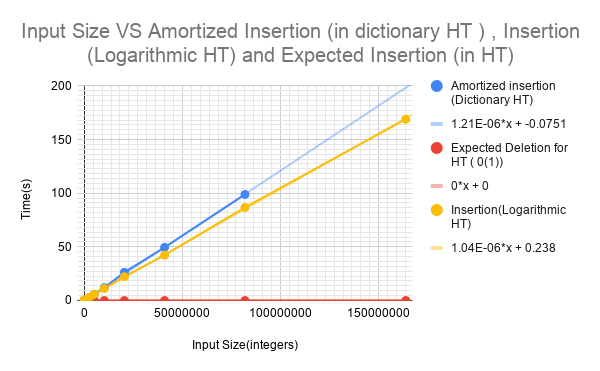
\includegraphics[height=\textwidth, width=\linewidth]{Insertion.png}
		\caption{Graph of Input Size Vs Insertion in both \\  Logarithmic and Dictionary Hash table}
		\label{fig:sub1}
	\end{subfigure}%
	\begin{subfigure}{.55\textwidth}
		\centering
		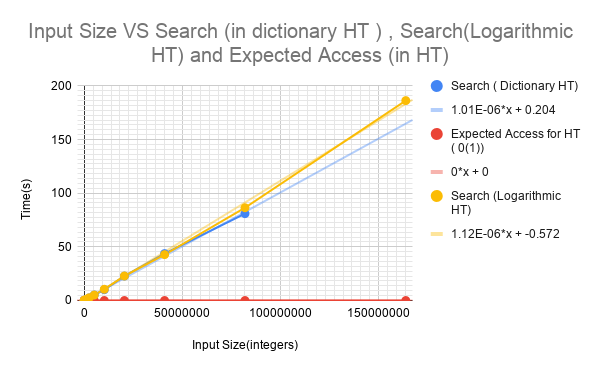
\includegraphics[height=\textwidth, width=\linewidth]{Search.png}
		\caption{Graph of Input Size Vs Search in both Logarithmic and Dictionary Hash table}
		\label{fig:sub2}
	\end{subfigure}
	\label{fig:test}
\end{figure}

\begin{figure}
	\centering
	\begin{minipage}{.55\textwidth}
		\centering
		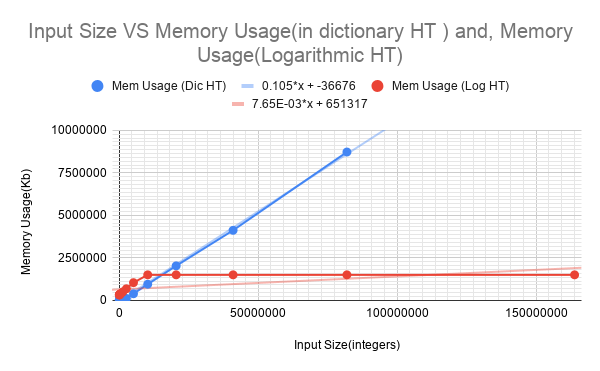
\includegraphics[height=\textwidth, width=\linewidth]{Memory.png}
		\caption{Graph of Input Size Vs Memory in\\ both  Hash table}
		\label{fig:test1}
	\end{minipage}%
	\begin{minipage}{.55\textwidth}
		\centering
		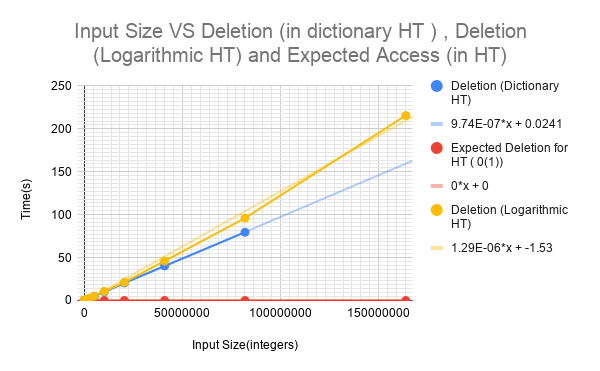
\includegraphics[height=\textwidth, width=\linewidth]{Deletion.png}
		\caption{Graph of Input Size Vs Search in both Logarithmic and Dictionary Hash table}
		\label{fig:test2}
	\end{minipage}
\end{figure}






\chapter{DISCUSSION}
\label{chap:DISCUSSION}
First, we observe from the data collected that, for the same input size the time complexities of the extendible hashing scheme differ from that of compact hashing scheme by a fraction of 1/100 of a second with the compact hashing scheme being slightly faster. Nonetheless, there is a noticeable difference in performance when the Input size become so large that there is a need to growth the table size. This growth in hash table size which is not part of the structure of compact-hashing need to be done by rehashing. Thus the time requirements for each rehashing, increase the time complexities of the dictionary hash table.\\
Moreover, in terms of space complexities, the logarithmic algorithm used a lot less memory compared to the dictionary algorithm. These difference in space requirement is because the dictionary hash table loads all data in memory meanwhile, the logarithmic algorithm indexes data on secondary storage. \\
Lastly, we can observe that there is no constant time in insertion, deletion and search irrespective of the Input size as expected from theoretical prediction. The reasons for this could be the fact that theoretical calculations do not account for the fact that as hash table size becomes very large, part of the table is moved out of memory to secondary disk(swap) to make available memory for other programs. This makes access time to this part of the table longer than expected. Usually 2 I/O operation 

In observing the space requirement on figure \ref{fig:test1}, we can predict a logarithmic grow in memory usage for the logarithmic hash table meanwhile, for the dictionary hash table there is a linear growth in memory usage for every rehash. Also, rehashing becomes very computationally costly as Input size increases.

\subsubsection{Key Applications }
When an exact match query is the most important, extendible hashing can be applicable (eg hash join).
Extendible hashing is also very applicable when the data to be hash is very large(eg a movie file) that it can not be loaded to the main memory. It is the backbone algorithm of most DBMS.
Compact-hashing is applicable when the Input size is not very large and each individual entry is small enough for a sufficient amount to be stored in memory.

\chapter{CONCLUSION} 
\label{chap:CONCLUSION}
We can conclude from our discussion that the time complexities of the dictionary and logarithmic hash tables deviate from their theoretical expectation, meanwhile the space complexities are as expected. Furthermore, there is a slight increase(a factor of 1/100 of a second) in performance of dictionary hash table in terms of insertion, search and deletion for individual operations but this performance degrades as input size increase and rehashing get involved making the logarithmic hash table overall faster. 

 \bigbreak
To improve the performance of the logarithmic method use, we could introduce the idea of elastic buckets. The extendible hashing scheme we used does not tolerate any overflow page. This can cause an increase significantly in directory size because one insertion could cause the directory to double many times. \\
To remedy this problem, we can introduce the idea of a bucket load factor( an idea proposed by Nabil I. Hachem \cite{hachem1993approximate} in his work on elastic bucket). After insertion we can check a bucket load factor: say greater than 100$\%$ before any doubling of a directory.



\backmatter
% bibliography, glossary and index would go here.
\addcontentsline{toc}{section}{References}
\renewcommand{\bibname}{References}
\printbibliography

\begin{appendices}
	\chapter{Some Appendix}
	 \section{Terms used to describe Extendible hashing} 
	 \textbf{Buckets}: They are a fixed size array into which  entries are stored.  Directories point to buckets. More than one directory can point to a bucket if its local depth is less than the global depth.\\
	 \textbf{Buckets size}: This is the amount of item that can be store in a bucket or the array size of a bucket.\\
	\textbf{Bucket Splitting}: When the number of elements in a bucket exceeds a particular size, then the bucket is split into two parts.\\
	\textbf{Buddy buckets}: This is a bucket referenced by the directory entry which shares the last (local depth - 1) bits. For instance, the buckets
		referenced by direction entries 1111 and 0111
		are buddy buckets.\\
	\textbf{Directories}: This is a list(array) of pointers pointing to buckets. Every index in this list has a unique id which may change each time when expansion takes place. The hash function hashes each entry to a directory id which is used to navigate to the appropriate bucket. \\	\textbf{Directory Expansion}: This occurs when a bucket overflows. When the local depth of the overflowing bucket is equal to the global depth, the directory expands.\\	
	\textbf{Global Depth}: This is the least significant bits of a binary representation of a hash. It is associated with the Directories. They denote the number of bits which are used by the hash function to categorize the keys. Global $Depth = Number$ of bits in directory index.\\
	\textbf{Local Depth}: It is the same as that of Global Depth except for the fact that Local Depth is associated with the buckets and not the directories. Local depth in accordance with the global depth is used to decide the action that to be performed in case an overflow occurs. Local Depth is always less than or equal to the Global Depth.\\
	\textbf{Load factor}: This is the ratio of the number of entries hash into the hash table to the key-space.
	\section{Terms related to Hashing schemes} 
	\textbf{Dynamic hashing}: In this hashing scheme the size of the hash table can be altered in as new entries are added or old ones deleted to avoid long overflow chains.  \\
	\textbf{Static hashing}: \label{app:static}  This is a hashing scheme were the number of buckets in the directory are fixed. When a bucket is full, we create (an) overflow bucket(s) by either linking to a shared overflow bucket or a linked list of overflow buckets.\\
	\textbf{In-memory access technique}: Access technique where the hash table is store in the RAM.\\
	\textbf{Disk-based access technique}: Access technique where the hash table stores it hashes on secondary storage and indexes them. The list of pointers indexing the hashes are store on RAM

\end{appendices}



\end{document}